
\documentclass[oneside,a4paper]{book}
%\pagestyle{headings}


%=============================================================================

\usepackage{amsthm}
\usepackage{xspace}
\usepackage{float}
\usepackage{ifthen}
\usepackage{amsbsy}
\usepackage{amssymb}
\usepackage{balance}
\usepackage{booktabs}
\usepackage{graphicx}
\usepackage{rotating}
\usepackage{multirow}
\usepackage{needspace}
\usepackage{microtype}
\usepackage{bold-extra}
\usepackage{geometry}
\usepackage{varioref}
\usepackage{xcolor}
\usepackage{textcomp}
\usepackage{listings}
\usepackage[normalem]{ulem} %emphasize still italic
\usepackage{ucs}
\usepackage{booktabs}

% \usepackage[utf8]{inputenc}
% \usepackage[htt]{hyphenat}
\usepackage{times}
\usepackage{url}
\usepackage{alltt}
\usepackage{amsmath}
\usepackage{xfrac}
\usepackage{subfigure}
\usepackage{appendix}
\usepackage{stmaryrd}   % for the \shortuparrow
\usepackage[utopia]{quotchap}

\usepackage{setspace}
\usepackage[numbers, sort&compress]{natbib}
\usepackage{mdwlist}        % support for better spaced lists
% allows for temporary adjustment of side margins
\usepackage{chngpage}
\usepackage[normalem]{ulem} 

% constants

\newcounter{qcounter}

% commands
\newcommand{\n}{$\cdot$}
\newcommand{\y}{\checkmark}
\newcommand{\subscript}[1]{$_{\textrm{\footnotesize{#1}}}$}
\newcommand{\superscript}[1]{$^{\textrm{\footnotesize{#1}}}$}
\newcommand{\vertical}[1]{\raisebox{-4em}{\begin{sideways}{#1}\end{sideways}}}

\newboolean{showedits}
\setboolean{showedits}{true} % toggle to show or hide edits
\ifthenelse{\boolean{showedits}}
{
       \newcommand{\ugh}[1]{\textcolor{red}{\uwave{#1}}} % please rephrase
       \newcommand{\ins}[1]{\textcolor{blue}{\uline{#1}}} % please insert
       \newcommand{\del}[1]{\textcolor{red}{\sout{#1}}} % please delete
       \newcommand{\chg}[2]{\textcolor{red}{\sout{#1}}{\ra}\textcolor{blue}{\uline{#2}}} % please change
}{
       \newcommand{\ugh}[1]{#1} % please rephrase
       \newcommand{\ins}[1]{#1} % please insert
       \newcommand{\del}[1]{} % please delete
       \newcommand{\chg}[2]{#2}
}


% ============================================================================
% Put edit comments in a really ugly standout display

\usepackage{xcolor}
\usepackage[normalem]{ulem}
\newcommand{\ra}{$\rightarrow$}


% comments \nb{label}{color}{text}
\newboolean{showcomments}
\setboolean{showcomments}{true}
\ifthenelse{\boolean{showcomments}}
    {\newcommand{\nb}[3]{
        {\colorbox{#2}{\bfseries\sffamily\scriptsize\textcolor{white}{#1}}}
        {\textcolor{#2}{\sf\small$\blacktriangleright$\textit{#3}$\blacktriangleleft$}}}
     \newcommand{\version}{\emph{\scriptsize$-$Id$-$}}
%	 \newcommand{\ugh}[1]{\textcolor{red}{\uwave{#1}}} % please rephrase
%	 \newcommand{\ins}[1]{\textcolor{blue}{\uline{#1}}} % please insert
%	 \newcommand{\del}[1]{\textcolor{red}{\sout{#1}}} % please delete
%	 \newcommand{\chg}[2]{\textcolor{red}{\sout{#1}}{\ra}\textcolor{blue}{\uline{#2}}} % please change
	 \newcommand{\chk}[1]{\textcolor{ForestGreen}{#1}} % changed, please check
	}
    {\newcommand{\nb}[3]{}
     \newcommand{\version}{}
	\newcommand{\chk}[1]{} % changed, please check
	}

% ============================================================================
% Make quotes be italic
\renewenvironment{quote}
    {\list{}{\rightmargin\leftmargin}%
     \item\relax\begin{it}}
    {\end{it}\endlist}

\newcommand{\ttimes}{\ensuremath{\times}}

%=============================================================================

\newcommand{\needlines}[1]{\Needspace{#1\baselineskip}}

% source code
\usepackage{xcolor}
\usepackage{textcomp}
\usepackage{listings}
\definecolor{source}{gray}{0.9}
\lstset{
	language={},
	% characters
	tabsize=3,
	upquote=true,
	escapechar={!},
	keepspaces=true,
	breaklines=false,
	alsoletter={:},
	breakautoindent=true,
	columns=fullflexible,
	showstringspaces=false,
	basicstyle=\footnotesize\ttfamily,
	% background
	frame=single,
    framerule=0pt,
	backgroundcolor=\color{source},
	% numbering
	numbersep=5pt,
	numberstyle=\tiny,
	numberfirstline=true,
	% captioning
	captionpos=b,
	numberbychapter=false,
	% formatting (html)
	moredelim=[is][\textbf]{<b>}{</b>},
	moredelim=[is][\textit]{<i>}{</i>},
	moredelim=[is][\uline]{<u>}{</u>}}
\newcommand{\ct}{\lstinline[backgroundcolor=\color{white},basicstyle=\footnotesize\ttfamily]}
\newcommand{\lct}[1]{{\small\tt #1}}


%----------------------------------------------------------------------------
% references
\newcommand{\tabref}[1]{\hyperref[{tab:#1}]{Table~\ref*{tab:#1}}}
\newcommand{\figref}[1]{\hyperref[{fig:#1}]{Figure~\ref*{fig:#1}}}
\newcommand{\secref}[1]{\hyperref[{sec:#1}]{Section~\ref*{sec:#1}}}
\newcommand{\lstref}[1]{\hyperref[{lst:#1}]{Listing~\ref*{lst:#1}}}
\newcommand{\charef}[1]{\hyperref[{cha:#1}]{Chapter~\ref*{cha:#1}}}
%----------------------------------------------------------------------------

% abbreviations
\tracingcolors 4
\setcounter{tocdepth}{3}
\setcounter{secnumdepth}{3}
\newcommand{\ie}{\emph{i.e.,}\xspace}
\newcommand{\eg}{\emph{e.g.,}\xspace}
\newcommand{\etc}{\emph{etc.}\xspace}
\newcommand{\etal}{\emph{et al.}\xspace}


\newcommand{\newevenside}{
	\ifthenelse{\isodd{\thepage}}{\newpage}{
	\newpage
        \phantom{placeholder} % doesn't appear on page
	\thispagestyle{empty} % if want no header/footer
	\newpage
	}
}

\def\stretchfactor{1}
\newcommand{\mychapter}[1]{\setstretch{1}
    \chapter{#1}\setstretch{\stretchfactor}}

%----------------------------------------------------------------------------
\newcommand{\lessSpace}{\vspace{-1em}}
\DeclareGraphicsExtensions{.pdf,.png}
\graphicspath{{images/}}
\newcommand{\fig}[4]{
	\begin{figure}[#1]
		\centering
		\includegraphics[width=#2\textwidth]{#3}
		\lessSpace
		\caption{\label{fig:#3}#4}
	\end{figure}}

% ===========================================================================


\newcommand{\thesistitle}{Automating high-quality translations for Mobile Apps}
\newcommand{\thesisauthor}{Wanzenried \& Stefan}
\newcommand{\thesisleiter}{Prof. Dr. Philippe Cudr\'{e}-Mauroux}
\newcommand{\thesisasst}{Roman Prokofyev}
\newcommand{\thesissubtitle}{}
\newcommand{\thesisdate}{May 2016}



% ===========================================================================

\usepackage[ colorlinks=true, urlcolor=black, linkcolor=black,
			citecolor=black, bookmarksnumbered=true, bookmarks=true,
			plainpages=false,
			pdftitle={\thesistitle}, pdfauthor={\thesisauthor},
			pdfsubject={\thesissubtitle}, pdfpagelabels]{hyperref}

\newcommand{\hrref}[2]{\hyperref}
% ===========================================================================
% ===========================================================================


% D O C U M E N T
% % % % % % % % % % % % % % % % % % % % % % % % % % % % % % % % % %
\begin{document}

% T I T L E
% % % % % % % % % % % % % % % % % % % % % % % % % % % % % % % % % %
\begin{titlepage}  
  \begin{center}  
  
  \begin{figure}[t]  
  \vspace*{-2cm}        % to move header logo at the top 
  \center{
\includegraphics[scale=0.2]{logos/MSc_quer.png}}
  \vspace{0.4in}     
  \end{figure}

    \thispagestyle{empty}
    
    {\bfseries\Huge \thesistitle \par
    \Large \vspace{0.1in} \thesissubtitle \par}

    \vspace{0.3in} 
    \LARGE{\textbf{Master Thesis} \\}
    \vspace{0.4in}

    {\Large \thesisauthor \par from \par Bern BE, Switzerland}
    
    \vspace{0.3in}
%    {\Large Home University \par}
    {\Large Philosophisch-naturwissenschaftliche Fakult\"{a}t \\
            der Universit\"{a}t Bern \par}
    \vfill
    {\Large \thesisdate \par}
    \vspace{0.3in}
    %Leiter der Arbeit: \par
%   {\Large \thesisleiter, Research Group, Institute, University, Supervisor}\par
   {\Large \thesisleiter, eXascale Infolab, University of Fribourg, Switzerland, Supervisor}\par
   {\Large \thesisasst, eXascale Infolab, University of Fribourg, Switzerland, Assistant}
  

  \vspace{0.9in}
 
  % === Logos ==============================================     
  \begin{figure}[htp]
    \centering
    
\includegraphics[scale=0.30]{logos/UNI_Bern.png}\hfill
    
\includegraphics[scale=0.30]{logos/UNI_Neuenburg.png}\hfill
    
\includegraphics[scale=0.80]{logos/UNI_Fribourg.png}
  \end{figure}
  % === // Logos ===========================================    


  \end{center}

\end{titlepage}


% A B S T R A C T
% % % % % % % % % % % % % % % % % % % % % % % % % % % % % % % % % %
\chapter*{\centering Abstract}
\begin{quotation}
\noindent 
Every day, hundreds of mobile applications are added to stores such as Google Play or AppStore. Many of them are intended to be used internationally, and thus require translation of the interface. At the same time, many more mobile apps already available for download in these stores. Leveraging the translation bases of existing applications, we could immediately provide high-quality translations for new apps without need to go though a human-translation process. 

This project aims to extract and parse translations of existing applications to see if they can be used to translate new ones. A prototype application allows to translate existing apps from a given source to a target language. Translations are generated with different algorithms in statistical machine translation.
\end{quotation}
\clearpage


% C O N T E N T S 
% % % % % % % % % % % % % % % % % % % % % % % % % % % % % % % % % % % % % % % %
\tableofcontents

%%%%%%%%%%%%%%%%%%%%%%%%%%%%%%%%%%
%%%% NEW CHAPTER %%%%%%%%%%%%%%%%%%%%%
%%%%%%%%%%%%%%%%%%%%%%%%%%%%%%%%%%
\chapter{Introduction}
\label{cha:introduction}

Android, iPhone and Windows smart phones are available in countries all over the world. If an app is intended to be used internationally, translating it into multiple languages can be important to attract users. Users may only use the app if its text is available in their native language. Offering multiple languages is therefore crucial for paid apps to increase sales. However, translating an app requires additional effort. From a developers perspective, all strings must be isolated in order to replace them with different values for each supported language. Furthermore, translating text itself is a difficult task which usually requires the work of a professional translator.

The main idea of this thesis is to collect a lot of existing apps and extract their translations. Are we able to provide high quality translations with the help of Statistical Machine Translation (SMT)? To reduce the scope of different mobile operating systems and languages, we focus on automatic translations of Android apps from English to French and German. From now on, the term \emph{app} in this thesis refers to a Android application. We have chosen French and German as target languages for the translations because they are natively spoken in Switzerland, which makes understanding the produced results easier. %Also our data analysis showed that these two languages are very popular.% 
SMT is the dominant approach in automating translations and used by services like ``Google Translate''\footnote{\url{https://translate.google.com}} and Microsoft's ``Bing Translator''\footnote{\url{https://www.bing.com/translator}}. In this thesis, we use different SMT algorithms to produce translations and compare their results, both manually and automatically. A prototype web application is built which serves as a playground to translate strings and apps.

\chapter{Problem Analysis}
\label{cha:problem_analysis}

This chapter answers the question why it is important to offer multiple languages for apps.  

%Furthermore we take a look at existing translation services and briefly introduce how the service developed with this thesis is going to work. %

\section{Importance of Translating Mobile Apps}

%https://web.archive.org/web/20150402231142/http://www.distimo.com/blog/2012_10_publication-the-impact-of-app-translations/%

%https://web.archive.org/web/20150327084808/http://www.distimo.com/publications%

Google encourages developers to localize their apps on their localization checklist.\footnote{Android localization checklist: \url{http://developer.android.com/distribute/tools/localization-checklist.html}}

\begin{quote}
Android and Google Play offer you a worldwide audience for your apps, with an addressable user base that's growing very rapidly in countries such as Japan, Korea, India, Brazil, and Russia. We strongly encourage you to localize as it can maximize your apps’ distribution potential resulting in ratings from users around the world.
\end{quote}

The developer should first identify the countries where the app will be distributed based on the overall market size and opportunity, app category, local pricing etc. According to the identified countries, the supported languages are determined. Ideally an app supports multiple languages already before the first version is available in the app store. Users may install the app only once and forget about it, if they are not able to understand it.

Since 2013, Google offers an (human-based) app translation service to developers.\footnote{Android Developers Blog post about Googles translation service: \url{http://android-developers.blogspot.ch/2013/11/app-translation-service-now-available.html}} Several developers who participated at the pilot program shared their results after translating their apps:

\begin{itemize}
\item The developers of Zombie Ragdoll\footnote{Game Zombie Ragdoll in the Google Playstore: \url{https://play.google.com/store/apps/details?id=com.rvappstudios.zombieragdoll}} used this tool to launch their new game simultaneously in 20 languages in August 2013. When they combined app translation with local marketing campaigns, they found that 80\% of their installs came from non-English-language users.
\item Dating app SayHi\footnote{Dating app SayHi! in the Google Playstore: \url{https://play.google.com/store/apps/details?id=com.unearby.sayhi}} Chat expanded into 13 additional languages using the App Translation Service. They saw 120\% install growth in localized markets and improved user reviews of the professionally translated UI.
\item The developer of card game G4A Indian Rummy\footnote{Card game Indian Rummy \url{https://play.google.com/store/apps/details?id=org.games4all.android.games.indianrummy.prod}} found that the App Translation Service was easier to use than their previous translation methods, and saw a 300\% increase with user engagement in localized apps.
\end{itemize}


In 2012, ``App Annie'' \footnote{\url{https://www.appannie.com}} (former called ``Distimo''), published a study where they analysed the impact of translations to iPhone apps.\footnote{App Annie's study The impact of app translations: \url{https://web.archive.org/web/20150327084808/http://www.distimo.com/publications}} They found out that the use of native language is still limited in several countries, for example Italy, Russia or Brazil. Native-only apps are mostly used in Asian countries (see Figure \ref{fig:problem_analysis_impact_languages}).
The study followed 200 iPhone apps that introduced native language support in a market and observed their growth. Only one week after the local language support was introduced with an app update, downloading increased by 128\% and revenue by 26\%.

%Another case-study by David Janner from make app magazine\footnote{\url{http://makeappmag.com/iphone-app-localization-keywords}} observed the impact of translating one single app.
%

\begin{figure}[H]
    \centering
    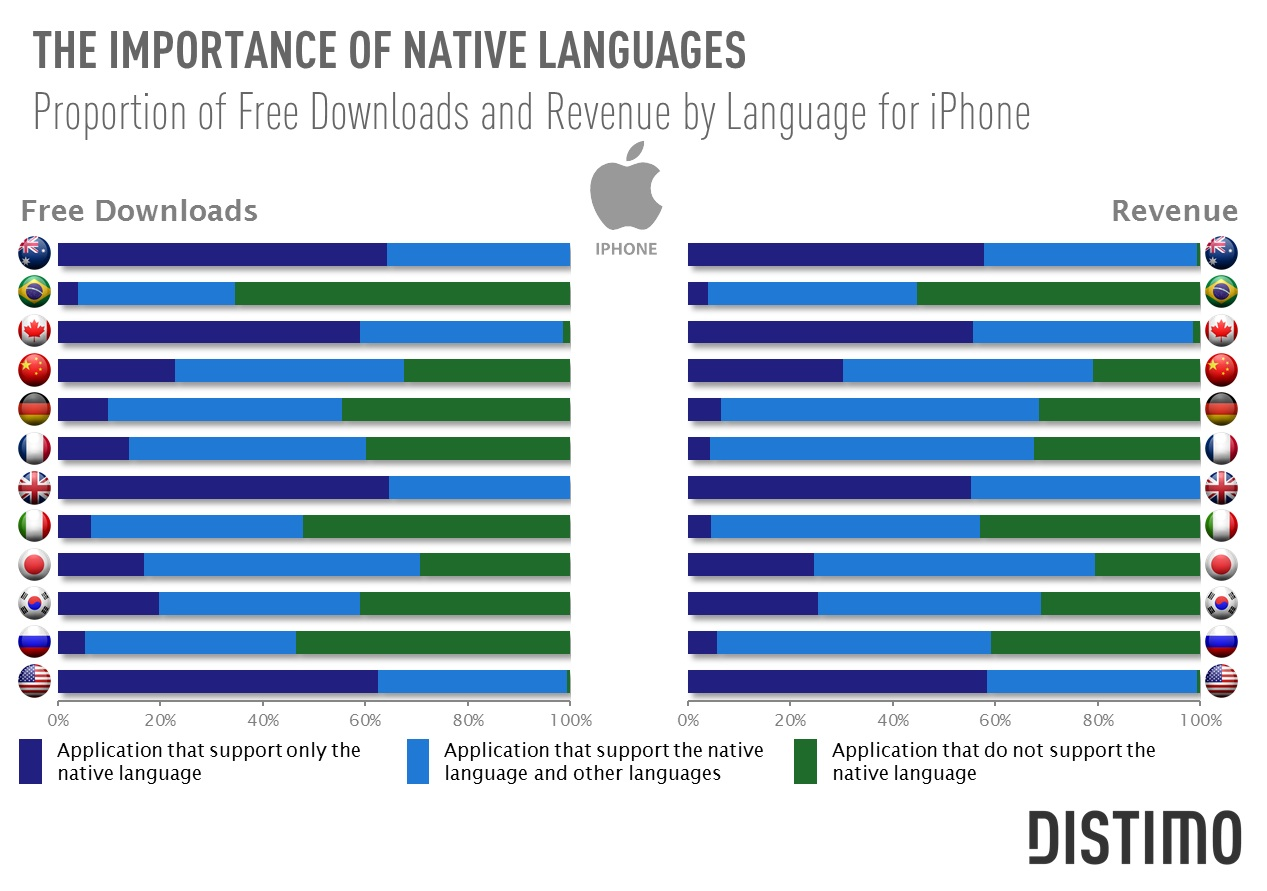
\includegraphics[width=0.8\textwidth]{images/problem_analysis_app_annie.jpg}
    \caption{Screenshot from the study ``The impact of app translations'' by App Annie showing the distribution of apps supporting native and other languages for the 12 top languages.}
    \label{fig:problem_analysis_impact_languages}
\end{figure}


\section{Translation Services}



\section{Statistical Machine Translation}

Machine translation has a long history, but over the last decade or two, its evolution has taken on a new direction - a direction that is mirrored in other subfields of natural language processing. This new direction is grounded in the premise that language is so rich and complex that it could never be fully analyzed and distilled into a set of rules, which are then encoded into a computer program. Instead, the new direction is to develop a machine that discovers the rules of translation automatically from a large corpus of translated text, by pairing the input and output of the translation process, and learning from the statistics over the data.\cite{smt_book_koehn}

%Statistical Machine Translation (SMT) is based on a large corpus of bilingual data. A translation model is trained to output the best possible translation according to some probabilistic function. In the context of this thesis it means that we learn a translation system from extracted translation of various apps.%

SMT translation models are usually trained on a large parallel corpus which is freely available on the web \footnote{\url{http://www.statmt.org/europarl/}}. The BLEU metric is then used to measure the quality of the produced translations. \cite{bleu_score}
There exists a recurring translation task of the ``Workshop on statistical machine translation'', which focuses on translating european language pairs by improving existing systems\footnote{\url{http://www.statmt.org/wmt15/translation-task.html}}.

In this thesis, we compare two different SMT algorithm and evaluate how they perform in the context of translating short sentences of mobile apps. The models are therefore applied on a much smaller data set than usual.

\section{Challenges}


\begin{itemize}
\item Quality of existing translations
\item Where and how to obtain large amount of apps
\item Hardware to train the translation models
\item How many data is needed to produce good results?
\item How can we measure good translations?
\end{itemize}



%\section{Android apps and internationalization}

%Android uses a key-value based approach to store translations and other resources in XML files\footnote{\url{http://developer.android.com/guide/topics/resources/localization.html}}. For each supported language, one XML file exists, containing the translated values to given keys. In the source code, a string is no longer hardcoded but referenced by a translation key.%

%\section{Challenges}%



\chapter{Related Work}
%In which we learn what have other done to address similar problems. For example, the work of Star \cite{Star89}

%Overview of SMT
%Has been done but not specific domain of short sentences mobile

This chapter provides an overview of Statistical Machine Translation (SMT). We consider two different models. The first one is called ``Statistical Phrase-Based Translation'' and was introduced in 2003 by Philipp Koehn et al. \cite{smt_phrase_based}\cite{smt_book_koehn} The second, more recent model, uses Deep Learning Neural Networks to perform translations. \cite{smt_deep_learning}

\section{Phrase-Based Machine Translation}

\subsection{Model}

Given the task to translate a sentence from a foreign language \(f = f_1, f_2, f_3..., f_m\) into an english sentence \(e = e_1, e_2, e_3 ..., e_n\), the translation model is based on the following probabilistic equation:

\[P(e|f)\]

To find the best english translation, the following equation is used (Bayes rule).

\[e_{best} = argmax_eP(e|f)\]
\[= argmax_e\frac{P(f|e)P(e)}{P(f)}\]
\[= argmax_e P(e|f)P(e)\]

where \(P(e)\) is called the \emph{language model} and \(P(f|e)\) is the \emph{translation model}.

The translation model is further decomposed:

\[p(\bar{f}_1^I|\bar{e}_1^I) = \prod_{i=1}^I \phi(\bar{f}_i^I|\bar{e}_i^I) d(start_i - end_{i-1} -1)\]

where \(\phi\) is called the \emph{phrase translation probability} and \(d\) is the \emph{reordering probability}.

The foreign sentence \emph{f} is broken up into \emph{I} phrases \(\bar{f}_i\). Each foreign phrase is translated into an English phrase \(\bar{e}_i\).

Reordering is handled by a \emph{distance based reordering model}. We define \(start_i\) as the position of the first word of the foreign input phrase that translates to the \emph{i}th English phrase, and \(end_i\) as the position of the last word of that foreign phrase. The reordering distance is the number of words skipped when taking foreign words out of sequence (see figure \ref{fig:related_work_phrase_based_reordering}).

\begin{figure}[H]
    \centering
    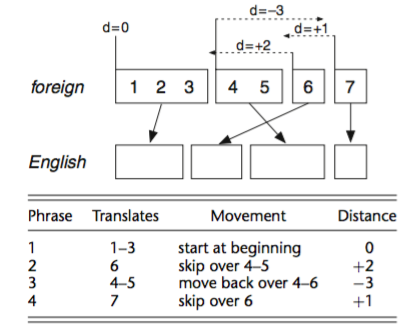
\includegraphics[width=0.4\textwidth]{images/related_work_phrase_based_reordering.png}
    \caption{Distance based reordering}
    \label{fig:related_work_phrase_based_reordering}
\end{figure}

\emph{d} is turned into a proper probability distribution by applying an exponentially decaying cost function \(d(x) = \alpha^{|x|}\) with \(\alpha \epsilon [0,1]\). This means that movements of phrases over large distances are more expensive than shorter movements or no movement at all.


\subsection{Learning a Phrase Translation Table}

Building a phrase translation table involves three stages:
\begin{enumerate}
\item \textbf{Word alignment} The words of each sentence from the parallel corpus of the foreign and English language must be aligned in order to extract phrase pairs. The alignment is typically done by using one of the IBM models.\footnote{IBM word alignment models: \url{https://en.wikipedia.org/wiki/IBM_alignment_models}} Figure \ref{fig:related_work_word_alignment} shows an example of word alignment for a top term from our corpus.
\item \textbf{Extraciton of phrase pairs} Extract all phrase pairs of parallel sentences that are consistent with word alignment.
\item \textbf{Scoring phrase pairs} Assign probabilities to phrase translations.
\end{enumerate}

\begin{figure}[H]
    \centering
    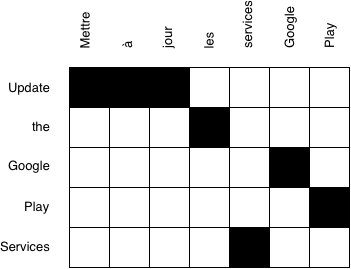
\includegraphics[width=0.3\textwidth]{images/related_work_word_alignment.png}
    \caption{Word alignment between a top term of our parallel Enlgish/French corpus.}
    \label{fig:related_work_word_alignment}
\end{figure}

\begin{figure}[H]
    \centering
    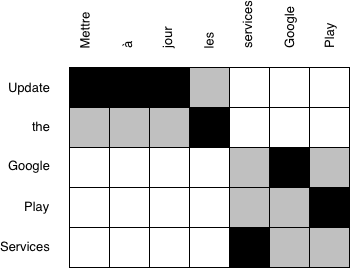
\includegraphics[width=0.3 \textwidth]{images/related_work_phrase_alignment.png}
    \caption{Extract phrase pairs consistent with word alignment.}
    \label{fig:related_work_phrase_alignment}
\end{figure}


We are able to extract the following phrase pairs from the example sentence:
\begin{itemize}
\item Update the Google Play Services / Mettre \a`a jour les services Google Play
\item Update / Mettre \a`a jour
\item Update the / Mettre \a`a jour les
\item Google Play Services / services Google Play
\item The Google Play Services / les services Google Play
\item Google Play / Google Play 
\end{itemize}

The last step is to estimate the phrase translation probabilities (scoring by relative frequency):

\[\phi(\bar{f}|\bar{e}) = \frac{count(\bar{e},\bar{f})}{\sum_{\bar{f}_i}count(\bar{e},\bar{f}_i)}\]


\subsection{Decoding}

- Search problem

\section{Deep Learning Neural Networks}


\chapter{Data Analysis}

\section{Apps}

A total of 698 free Android apps were collected from various categories\footnote{Click on Categories to see a list of available categories at:  \url{https://play.google.com/store/apps?hl=en}}, ensuring a good mix of different translations. Most of them were chosen randomly beside the top apps, mostly from Google. Figure \ref{fig:data_analysis_top_apps_en} shows the top ten apps according to the number of available english translations. Note that the counts indicate the number of effective translations after eliminating uninteresting data during pre-processing the corpus (see chapter \ref{cha:data_extraction_prep_storage}). Most of the apps have similar counts for all the three languages. Surprisingly, some apps provide more translations for german and french than english. Different counts can happen because of:

\begin{enumerate}
\item Not all strings were translated to all languages. Some english words remain the same in the target language and don't need to be translated, e.g. E-Mail.
\item The XML files containing the translations are out of sync, e.g. the developer forgot to add a french translation.
\item Some translations were abandoned during pre-processing.
\end{enumerate}

34 apps did not isolate their strings in XML files (we assume that they are hardcoded in the programming code). This leaves a effective number of 664 apps where we could extract translations. However, 241 apps among them were not multilingual and therefore not useful for building translation systems. Unfortunately, apps are not marked as multi-language in the app store, so we only know if there are translations available after downloading and extracting the data.

\begin{figure}[H]
    \centering
    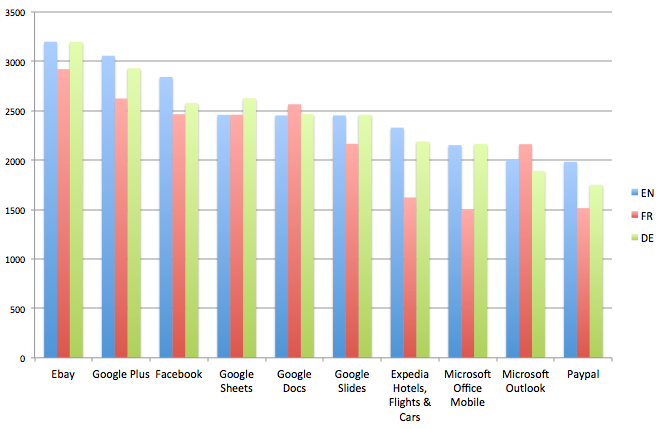
\includegraphics[width=0.75\textwidth]{images/data_analysis_top_apps_en.png}
    \caption{Top apps by the number of english translations}
    \label{fig:data_analysis_top_apps_en}
\end{figure}


\section{Languages}

We collected a total of 423 multilingual apps, offering its content at least for two languages. Figure \ref{fig:data_analysis_n_langs} shows the number of apps for the ten most used languages. French and German, where we focus on this thesis, are both in the top 4. The top apps are translated in many more languages. Overall, 117 different languages were available.

\begin{figure}[H]
    \centering
    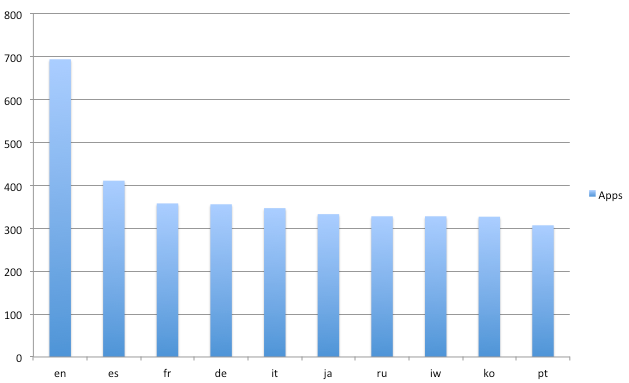
\includegraphics[width=0.75\textwidth]{images/data_analysis_languages_count.png}
    \caption{Number of apps available in the top ten languages.}
    \label{fig:data_analysis_n_langs}
\end{figure}


\section{Top Terms}


\begin{table}[H]
\centering
\resizebox{\textwidth}{!}{%
\begin{tabular}{@{}llllllll@{}}
\toprule
EN & Count &  & FR & Count &  & DE & Count \\ \midrule
Cancel & 1894 &  & Annuler & 1067 &  & Abbrechen & 886 \\
Done & 1230 &  & Supprimer & 745 &  & Google Play-Dienste aktivieren & 730 \\
Settings & 1102 &  & Connexion & 745 &  & Google Play-Dienste installieren & 728 \\
Search & 884 &  & Mettre à jour & 486 &  & Anmelden & 664 \\
Delete & 704 &  & Rechercher & 485 &  & Löschen & 664 \\
Enable Google Play services & 692 &  & Paramètres & 450 &  & Aktualisieren & 652 \\
Get Google Play services & 690 &  & Mettre à jour les services Google Play & 370 &  & Einstellungen & 569 \\
Log Out & 556 &  & Activer services google Play & 368 &  & Fertig & 548 \\
Update & 545 &  & Activer les services Google Play & 366 &  & Weiter & 484 \\
Share & 541 &  & Installer les services Google Play & 366 &  & Schliessen & 428 \\ \bottomrule
\end{tabular}
}
\caption{Top ten terms for english, french and german}
\label{table:data_analysis_top_terms}
\end{table}

\chapter{Data Extraction, Preparation and Storage}
\label{cha:data_extraction_prep_storage}

\section{Extract Translations}

An Android app has the form of a single binary file (suffix .apk). The XML files containing the translations are packed inside the .apk file. We used a software called ``Apktool''\footnote{\url{http://ibotpeaches.github.io/Apktool/}} to reverse engineer existing apps and extract the needed XML files.

\begin{figure}[H]
    \centering
    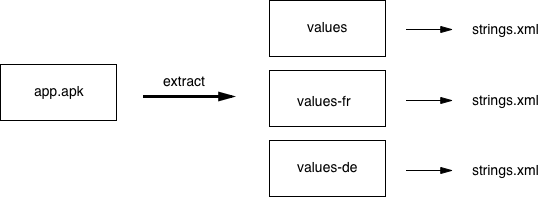
\includegraphics[width=0.6\textwidth]{images/data_extraction_xml.png}
    \caption{For each language, the translations are stored in a XML file}
    \label{fig:data_extraction_xml}
\end{figure}

Inside the \texttt{strings.xml} files, translations are stored key-value based. Each string has a unique key which holds the translation value for each language. Here is an example how an English XML file looks like:

\begin{verbatim}
<?xml version="1.0" encoding="utf-8"?>
<resources>
    <string name="close_app">Close Application</string>
    <string name="back">Back</string>
    ...
</resources>
\end{verbatim}


\section{Preprocess Translations}

This task involves two parts. First of all, the translations are sanitized from unwanted information such as HTML tags. Some strings are omitted at this stage because they do not provide any meaningful value to the translation process, for example URLs or string placeholders. Secondly, the sanitized strings are tokenized so that they can be used by an SMT system.

\subsection{Sanitizing}

The following rules are used to get rid of unwanted translations or parts of it:

\begin{itemize}
\item Trim the string from newlines (\texttt{\textbackslash n}), tabs (\textbackslash t) or carriage return (\textbackslash r)
\item Strip any HTML tags
\item Omit strings that are URLs (starting with http or www)
\item Remove strings placeholders like \texttt{\%s} or \texttt{\%1\$s}
\item Ignore words with less than 3 characters
\item Finally, the resulting string is trimmed again from spaces and must contain at least one alphanumerical character
\end{itemize}


\subsection{Tokenization and Truecasing}

Tokenization is required to separate words from punctuation. Each token is separated by a space character: ``\texttt{Hi, my name is John.}'' becomes ``\texttt{Hi , my name is John .}''

After tokenizsation, truecasing was applied to our text corpus.\footnote{\url{https://en.wikipedia.org/wiki/Truecasing}} In contrast to lowercasing, truecasing determines the proper capitalization of words. This is done by first analyzing all data and then apply the most likely capitalization. It is especially useful for words starting a sentence, that are written uppercase in many languages. For example the word ``\texttt{This}'' starting a sentence will become ``\texttt{this}'', because it is usually written lowercase.


\section{Data storage}


\subsection{Parallel and Monolingual Corpus}

After pre-processing the translations, they are written to text files, one sentence per line. The corpus is split into parallel and monolingual data. A parallel corpus (often also called bitext) describes sentence aligned text-files of one language pair. All sentences must be aligned so that line x of the translation source language corresponds to line x of the target language. The sentences are shuffled before writing to get a random mix of translations of different apps. Most SMT system use this parallel data to train their translation model, so the parallel corpus can be reused multiple times.

In addition, data of any language is also stored monolingual. All sentences of one language are written into a single text file. This is for example used to build language models, which are an important part of a phrase-based translation model (see chapter xy).

\subsection{Apache Solr}

We needed a simple way to store all translations, preferably with additional meta data, to perform data analysis and calculate statistics.
Apache Solr\footnote{\url{http://lucene.apache.org/solr/}} is used for this purpose. Solr is an open source text search platform built on top of Apache Lucene\footnote{\url{https://lucene.apache.org/core/}}. It allows to store the translations with additional meta data, such as the translation key and a unique app ID. Due to its way of indexing text data, Solr is very fast when querying for translation strings. Furthermore, built in tools allow to get nice statistics, for example the top terms grouped by language.

Solr is also used as Baseline translation system (see chapter xy).

\subsubsection{Setup and Schema}

Solr offers so called ``Cores'' where each core manages a separate index, schema and configuration\footnote{\url{https://cwiki.apache.org/confluence/display/solr/Solr+Cores+and+solr.xml}}. In our setup we created one core per language and one document per translation string. The schema is identical for each core (language) and consist of the following fields:

\begin{itemize}
\item \textbf{id} Unique ID used by Solr to identify a document.
\item \textbf{app\_id} Each app must have a unique app-ID.
\item \textbf{key} The translation key from the XML file.
\item \textbf{value} The translation value corresponding to the above key.
\item \textbf{value\_lc} Again the translation value, additionally indexed with a special start- and ending delimiter. This allows to search for exact values.
\end{itemize}

\begin{figure}[H]
    \centering
    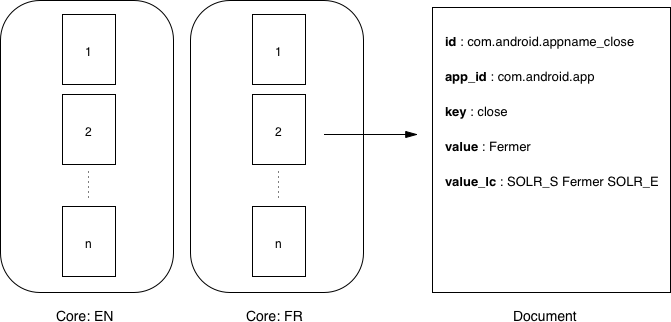
\includegraphics[width=0.8\textwidth]{images/data_extraction_solr_schema.png}
    \caption{Translations are stored in a document inside a separate Core per language}
    \label{fig:data_extraction_solr_schema}
\end{figure}

The data in the \texttt{value} and \texttt{value\_lc} fields is stored tokenized and lowercased. The Solr Standard Tokenizer\footnote{\url{https://cwiki.apache.org/confluence/display/solr/Tokenizers\#Tokenizers-StandardTokenizer}} splits text into tokens, treating whitespace and punctuation as delimiters. Delimiter characters are discarded.

\subsubsection{Queries}

\chapter{Translation Process}

\section{Baseline System}

\section{Moses}

\section{Tensorflow}

\chapter{Web Application}

The main purpose of the web application is to offer a simple way of testing the different implemented translation systems (Baseline with Solr, Moses and Tensorflow). However, the application could already be used by app developers to translate their XML translation files.

The interface allows to translate either plain strings or a XML translation file from one language to another. Each decoder offers some specific settings where the user can influence the decoder.

\section{Architecture}

% com.ancestry.android.apps.ancestry_your_capitalized
% com.google.android.apps.plus_collexion_abuse_appeal_rejected
% com.google.android.apps.plus_collexion_suspension_details
% --data_binary '{"id":"com.google.android.apps.plus_collexion_abuse_appeal_rejected","value":{"set":"votre"},"value_lc":{"set":"votre"}}'


\section{Frontend}

\chapter{Evaluation}


\section{BLEU Score}

\section{T}


%\chapter{The Problem}
%In which we understand what the problem is in detail.
%
%\chapter {The Solution}
%In which you describe your solution.
%
%\chapter {The Validation}
%In which you show how well the solution works.
%
%\chapter {Conclusion and Future Work}
%In which we step back, have a critical look at the entire work, then conclude, and learn what lies beyond this thesis.





%END Doc
%-------------------------------------------------------

\bibliography{thesis}
\bibliographystyle{plain}


\end{document}
